\documentclass[12pt]{article}
\usepackage{enumerate, hyperref}
\usepackage{amsmath, amssymb}
\usepackage[margin=1.1in]{geometry}
\usepackage{graphicx}
\linespread{1.2}



\begin{document}

\section{Marginal Likelihood}
The marginal likelihood changes slightly from simulation to simulation. Usually these deviations are relatively small, however, they do change the order because top models are fairly close to each other.
Below are two tables of $nu = 6$ (this was the best value according to the big run). One table is the same that was already reported, the second one is based on the same code but the random seed is set differently. \\
Take off: We may want to increase the number of draws. \\
\begin{table}[!ht]
	\centering
	\footnotesize
	\begin{tabular}{ccc}
		\hline
		Model & DF & log margLike \\ 
		\hline
		MOM + Mkt.RF + HML + RMW + CMA + QMJ + ME + ROE & 6 & 9690.48 \\ 
		MOM + Mkt.RF + HML + RMW + CMA + QMJ + ME + ROE + HMLDev & 6 & 9688.97 \\ 
		MOM + Mkt.RF + SMB + HML + RMW + CMA + QMJ + ME + HMLDev & 6 & 9688.84 \\ 
		MOM + Mkt.RF + SMB + HML + RMW + CMA + QMJ + ME & 6 & 9688.67 \\ 
		MOM + Mkt.RF + SMB + HML + RMW + CMA + QMJ + ROE & 6 & 9688.05 \\ 
		MOM + Mkt.RF + HML + RMW + CMA + QMJ + ME + IA & 6 & 9687.62 \\ 
		MOM + Mkt.RF + HML + RMW + CMA + QMJ + ME + IA + ROE & 6 & 9687.34 \\ 
		MOM + Mkt.RF + SMB + HML + RMW + CMA + QMJ + ME + IA & 6 & 9687.32 \\ 
		MOM + Mkt.RF + SMB + HML + RMW + CMA + QMJ + ROE + HMLDev & 6 & 9687.23 \\ 
		MOM + Mkt.RF + HML + RMW + CMA + QMJ + ME & 6 & 9687.13 \\ 
		constant + MOM + Mkt.RF + HML + RMW + CMA + QMJ + ME + ROE & 6 & 9687.09 \\ 
		MOM + Mkt.RF + SMB + HML + RMW + CMA + QMJ + ME + ROE & 6 & 9686.84 \\ 
		MOM + Mkt.RF + HML + RMW + CMA + QMJ + ME + IA + HMLDev & 6 & 9686.56 \\ 
		constant + MOM + Mkt.RF + HML + RMW + CMA + QMJ + ME + ROE + HMLDev & 6 & 9686.18 \\ 
		MOM + Mkt.RF + HML + RMW + CMA + QMJ + ME + HMLDev & 6 & 9686.1 \\ 
		\hline
	\end{tabular}
	\caption{Best Models (alternative run, only for $\nu = 6$)}
\end{table}
\begin{table}[!ht]
	\centering
	\footnotesize
	\begin{tabular}{ccc}
		\hline
		Model & DF & log margLike \\ 
	 \hline
	 MOM + Mkt.RF + HML + RMW + CMA + QMJ + ME + ROE & logML & 9690.77 \\ 
	 MOM + Mkt.RF + SMB + HML + RMW + CMA + QMJ + ROE & logML & 9689.14 \\ 
	 MOM + Mkt.RF + SMB + HML + RMW + CMA + QMJ + ME & logML & 9688.97 \\ 
	 MOM + Mkt.RF + HML + RMW + CMA + QMJ + ME + ROE + HMLDev & logML & 9688.26 \\ 
	 MOM + Mkt.RF + SMB + HML + RMW + CMA + QMJ + ME + HMLDev & logML & 9687.89 \\ 
	 MOM + Mkt.RF + HML + RMW + CMA + QMJ + ME + IA & logML & 9687.56 \\ 
	 constant + MOM + Mkt.RF + HML + RMW + CMA + QMJ + ME + ROE & logML & 9687.49 \\ 
	 MOM + Mkt.RF + SMB + HML + RMW + CMA + QMJ + ME + IA & logML & 9687.38 \\ 
	 MOM + Mkt.RF + HML + RMW + CMA + QMJ + ME + IA + ROE & logML & 9687.36 \\ 
	 MOM + Mkt.RF + SMB + HML + RMW + CMA + QMJ + ROE + HMLDev & logML & 9686.98 \\ 
	 MOM + Mkt.RF + SMB + HML + RMW + CMA + QMJ + ME + IA + HMLDev & logML & 9686.83 \\ 
	 MOM + Mkt.RF + HML + RMW + CMA + QMJ + ME & logML & 9686.17 \\ 
	 constant + MOM + Mkt.RF + HML + RMW + CMA + QMJ + ME + ROE + HMLDev & logML & 9686.11 \\ 
	 MOM + Mkt.RF + SMB + HML + RMW + CMA + QMJ + ME + ROE & logML & 9685.83 \\ 
	 constant + MOM + Mkt.RF + SMB + HML + RMW + CMA + QMJ + ROE & logML & 9685.82 \\ 
	 \hline
	\end{tabular}
		\caption{Best Models (original run, only for $\nu = 6$)}
\end{table} \\
When looking into the table in greater details, one can see that most changes are fairly modest: e.g for MOM + Mkt.RF + SMB + HML + RMW + CMA + QMJ + ME + HMLDev the marginal likelihood changed from 9687.89 to 9688.84. However, they do influence the order.\\
The exact reasons of this instability are so far undetermined. Keeping the training sample results fixed, the resulting value does not change up to the first digit (e.g. you may get 9690.728 and 9690.746 but not 9690.446). This means that it's not due to the second step estimation only or likelihood calculation itself. However, if both the training sample and the full sample results are re-simulated, these small changes accumulate, resulting into more significant differences. List of possible issues:
\begin{enumerate}
	\item Insufficient number of draws (currently using 10000). Increasing the number of draws is conceptually easy but increases the computation time.
	\item Computational instability with inverse Wishart draws (what we've see before). After inspecting the table below I don't think that's an issue: all components of the marginal log likelihood change. 
	\item These models are actually so similar?
\end{enumerate}
\begin{table}[]
	\centering

	\label{my-label}
	\begin{tabular}{cccc}
		& trial 1 & trial 2 (same training sample priors as 1) & trial 3 (re-simulate everything)\\
		\hline
prior  & -448.4318 & -448.3919 & -448.2381 \\
liki   & 9977.269  & 9977.171  & 9977.468  \\
post   & -161.8906 & -161.9668 & -161.9754 \\
marg L & 9690.728  & 9690.746  & 9691.205 
	\end{tabular}
		\caption{Example: changes in values after re-simulation}
\end{table}

\section{Comparison with ML}
In order to make sure that the posterior moments are sensible, we compare the results with a simple ML (not SUR). The posterior means are expected to be reasonably similar to the ML estimates. The results below are for the best model. \\
(Note: Our procedure does not return the draws for all models, that would not be efficient, so I repeated the simulation to get the draws. The log marginal likelihood is a little different. I didn't come up with a good way of representing that for a $10 \times 8$ vector of loadings and $5 \times 6 / 2 = 55$ elements of covariance matrix). Below are plots of different elements.\\
First, we explore the vector of factor loadings $\gamma$. The first picture plots posterior means and ML estimates. They are not identical but close enough. 
\begin{figure}[!h]
	\centering
	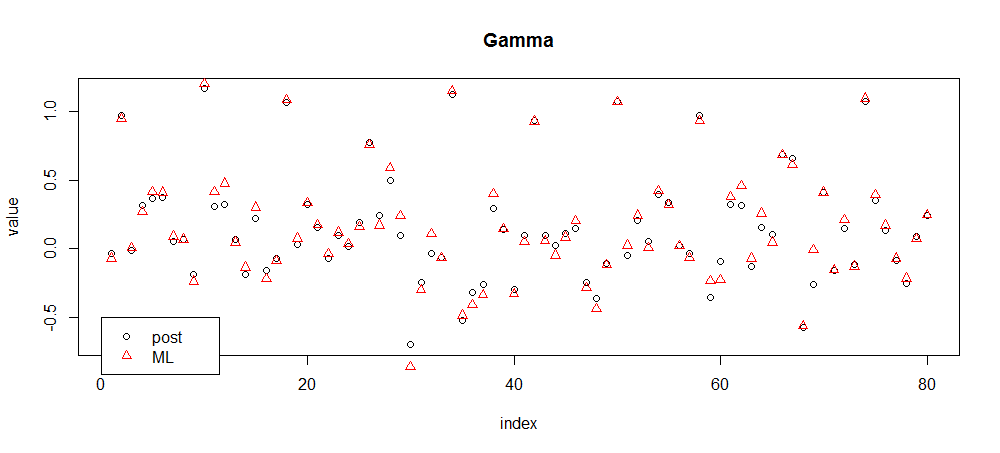
\includegraphics[width=15cm]{Pics/SanityCheckGamma.png}
	\caption{$\gamma$: posterior means vs. ML estimates}
\end{figure}
The posterior means are significantly updated in comparison with the priors but the values are in the same range.
\begin{figure}[!h]
	\centering
	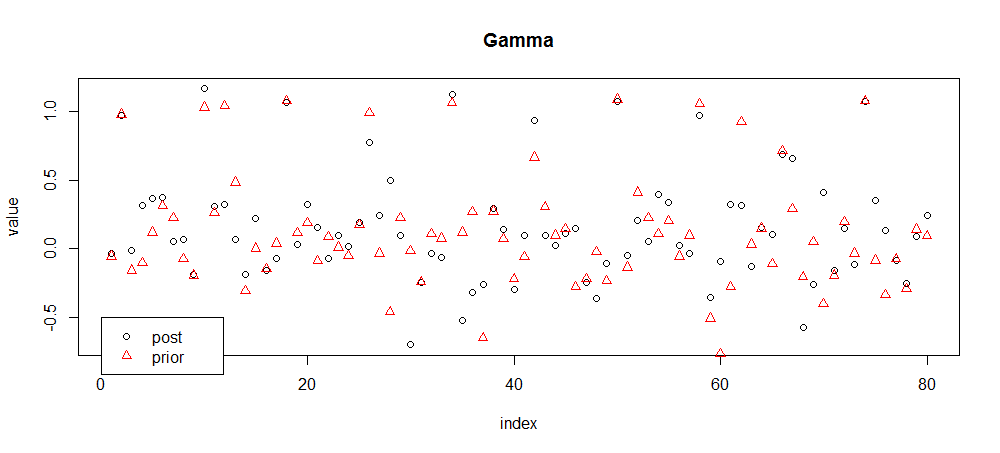
\includegraphics[width=15cm]{Pics/SanityCheckGammaPrior.png}
	\caption{$\gamma$: posterior means vs. second stage priors coming from the training sample}
\end{figure}
We can conclude that the draws of the parameter vector are reasonable. \\
Finally, compare the draws for the errors covariance matrix ($\Sigma$). Note that for Student-t distribution with 6 degrees of freedom the covariance matrix is a scaled version of the scale matrix $\Omega$: $\Sigma = \frac{\nu}{\nu - 2}\Omega = \frac{6}{4}\Omega$. We approximate the scale matrix $\Omega$ as the inverse of the posterior means of sample draws of $\Omega^{-1}$. 
\begin{figure}[!h]
	\centering
	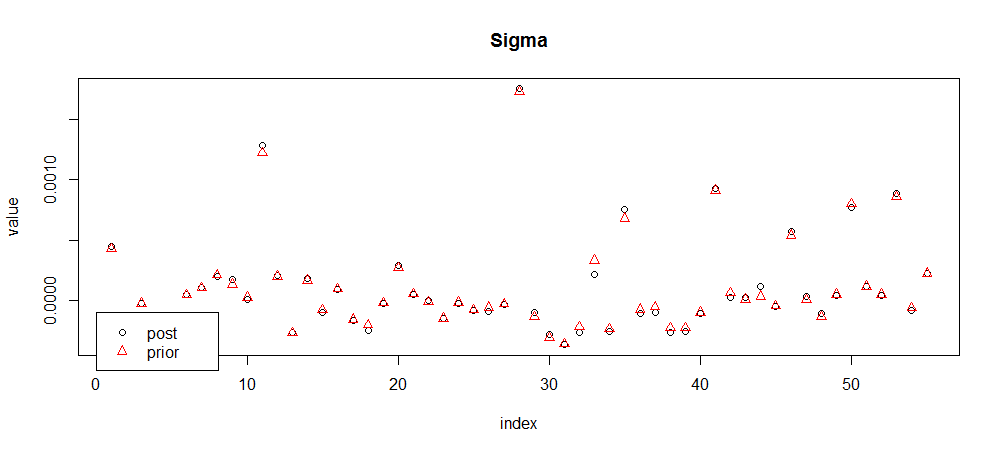
\includegraphics[width=15cm]{Pics/SanityCheckSigma.png}
	\caption{$\Sigma$: posterior means vs. ML}
\end{figure}
Again, the results from two methods are similar, so we conclude that the procedure produces reasonable estimates of the parameters of interest.
\end{document}
